\documentclass[./main.tex]{subfiles}

\begin{document}

\newcommand{\mockupdimension}{0.36\textwidth}

\subsection{Mockups}
This section contains the most significant mockups of our application. Some of them were already shown in the RASD document but they are included again to improve readability. 

\vfill
\begin{figure}[h]
    \begin{minipage}[t]{\mockupdimension}
        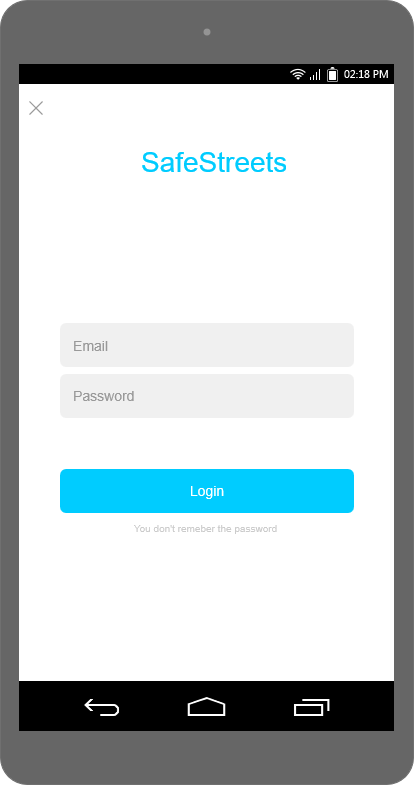
\includegraphics[width=\textwidth]{resources/Mockups/login}
        \caption{The login process for all types of users.}
        \label{fig:login}
    \end{minipage}
    \hfill
    \begin{minipage}[t]{\mockupdimension}
        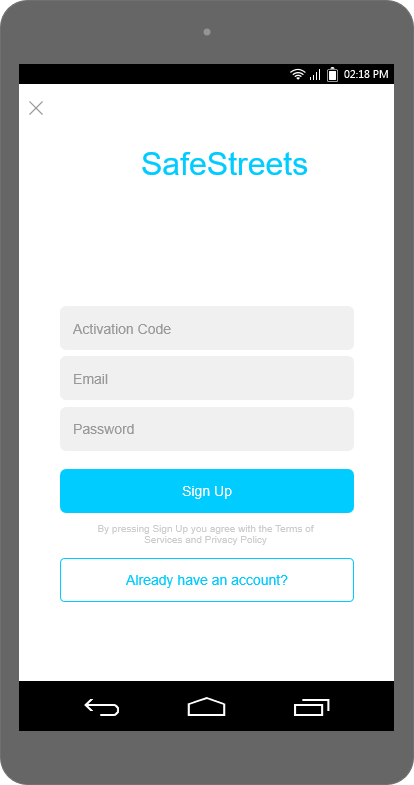
\includegraphics[width=\textwidth]{resources/Mockups/sign_up}
        \caption{The sign-up process for the authority/municipality user.}
        \label{fig:signup}
    \end{minipage}
\end{figure}
\vfill

\clearpage

\begin{figure}
    \centering
    \begin{minipage}[t]{\mockupdimension}
        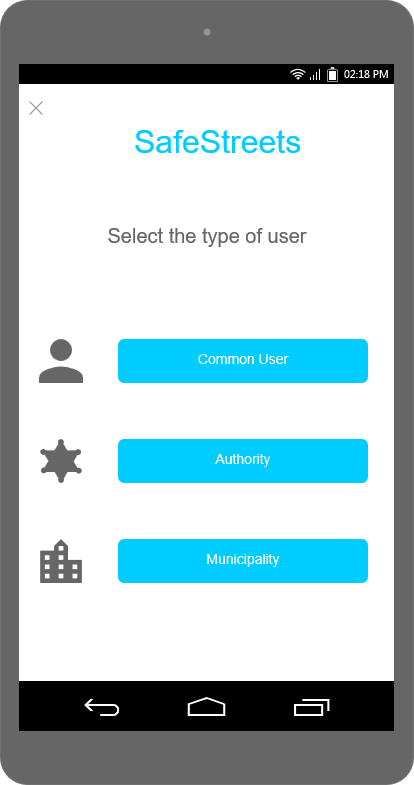
\includegraphics[width=\textwidth]{resources/Mockups/select_user}
        \caption{The choice between different types of users.}
        \label{fig:select_user}
    \end{minipage}
    \hfill
    \begin{minipage}[t]{\mockupdimension}
        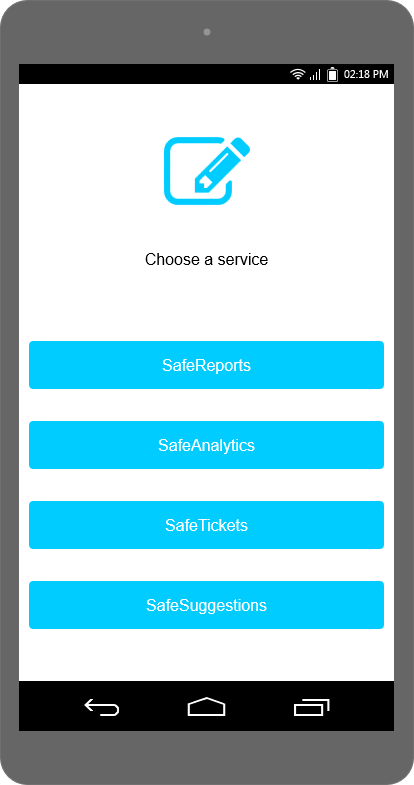
\includegraphics[width=\textwidth]{resources/Mockups/menu}
        \caption{The menu page. The available services depend on the type of user
                 as shown in the UX diagrams. }
        \label{fig:menu}
    \end{minipage}
\end{figure}


\begin{figure}
    \centering
    \begin{minipage}[t]{\mockupdimension}
        \footnotesize
        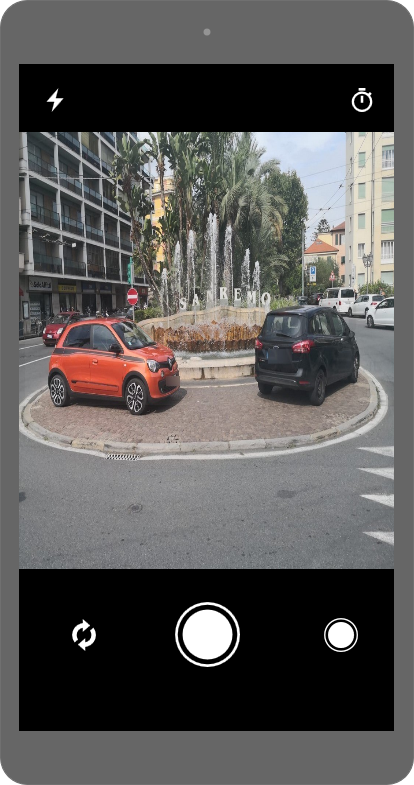
\includegraphics[width=\textwidth]{resources/Mockups/picture}
        \caption{Take picture process.}
        \label{fig:picture}
    \end{minipage}
    \hfill
    \begin{minipage}[t]{\mockupdimension}
        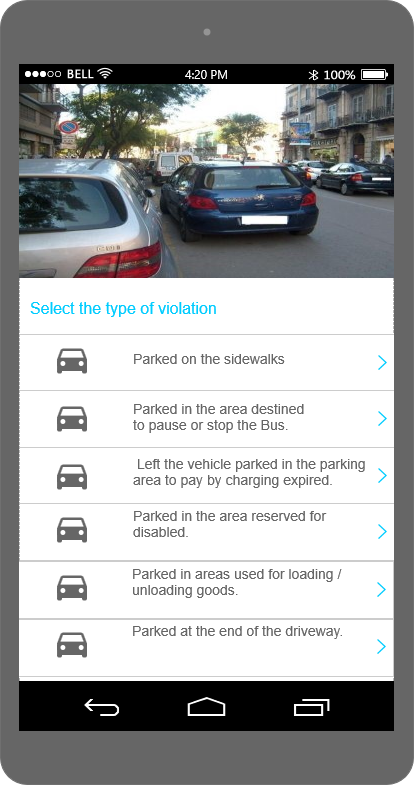
\includegraphics[width=\textwidth]{resources/Mockups/select_violation}
        \caption{The user needs to select the violation.}
        \label{fig:select_violation}
    \end{minipage}
\end{figure}

\clearpage

\begin{figure}
    \centering
    \begin{minipage}[t]{\mockupdimension}
        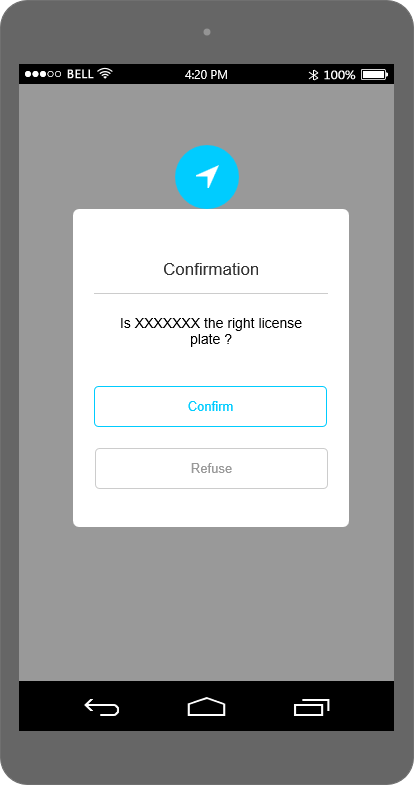
\includegraphics[width=\textwidth]{resources/Mockups/user_confirmation}
        \caption{The user needs to confirm the license plate. }
        \label{fig:user_confirmation}
    \end{minipage}
    \hfill
    \begin{minipage}[t]{\mockupdimension}
        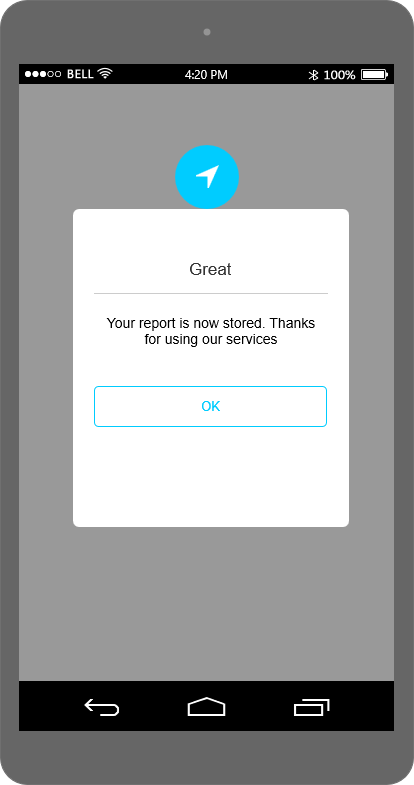
\includegraphics[width=\textwidth]{resources/Mockups/reports_stored}
        \caption{Confirmation of a successful report.}
        \label{fig:reports_stored}
    \end{minipage}
\end{figure}

\begin{figure}
    \centering
    \begin{minipage}[t]{\mockupdimension}
        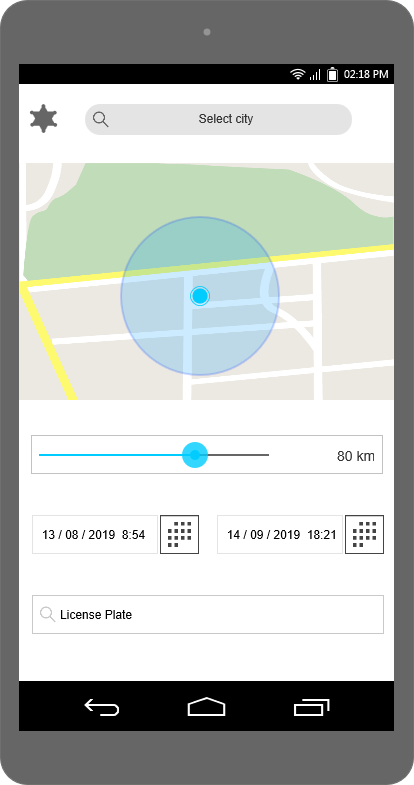
\includegraphics[width=\textwidth]{resources/Mockups/filter1}
        \caption{Filters. As shown in the UX diagram different users and services requires different                                                   filters}
        \label{fig:filter1}
    \end{minipage}
    \hfill
    \begin{minipage}[t]{\mockupdimension}
        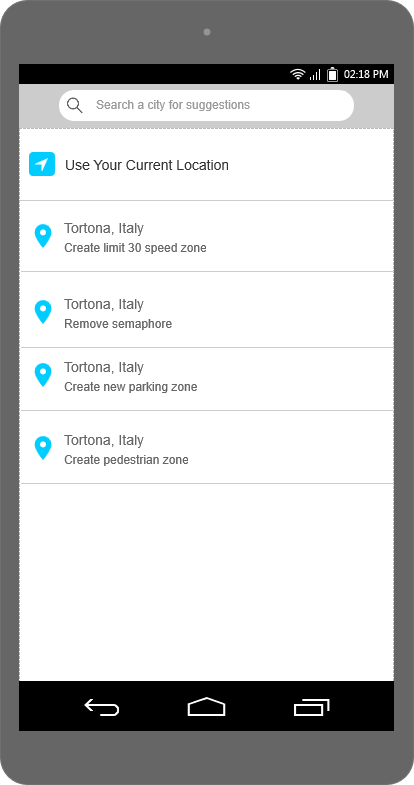
\includegraphics[width=\textwidth]{resources/Mockups/suggestions}
        \caption{The results of a SafeSuggestions query.}
        \label{fig:suggestions}
    \end{minipage}
\end{figure}

\clearpage

\begin{figure}
    \centering
    \begin{minipage}[t]{\mockupdimension}
        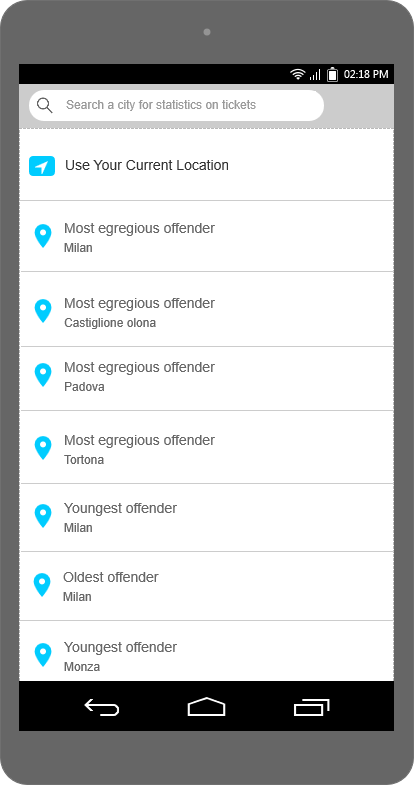
\includegraphics[width=\textwidth]{resources/Mockups/tickets_statistics}
        \caption{The results of a SafeTickets query.}
        \label{fig:ticket_statistics}
    \end{minipage}
    \hfill
    \begin{minipage}[t]{\mockupdimension}
        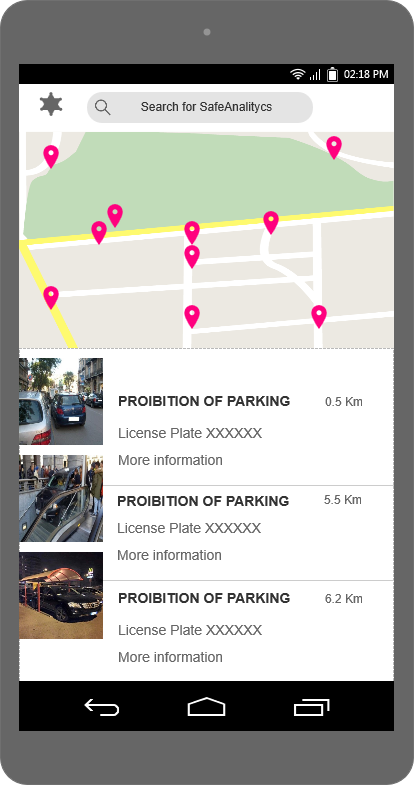
\includegraphics[width=\textwidth]{resources/Mockups/analytics_results}
        \caption{The results of a SafeAnalytics query.}
        \label{fig:analytics_results}
    \end{minipage}
\end{figure}


\clearpage

\subsection{UX diagrams}

\begin{figure}[H]
\centering
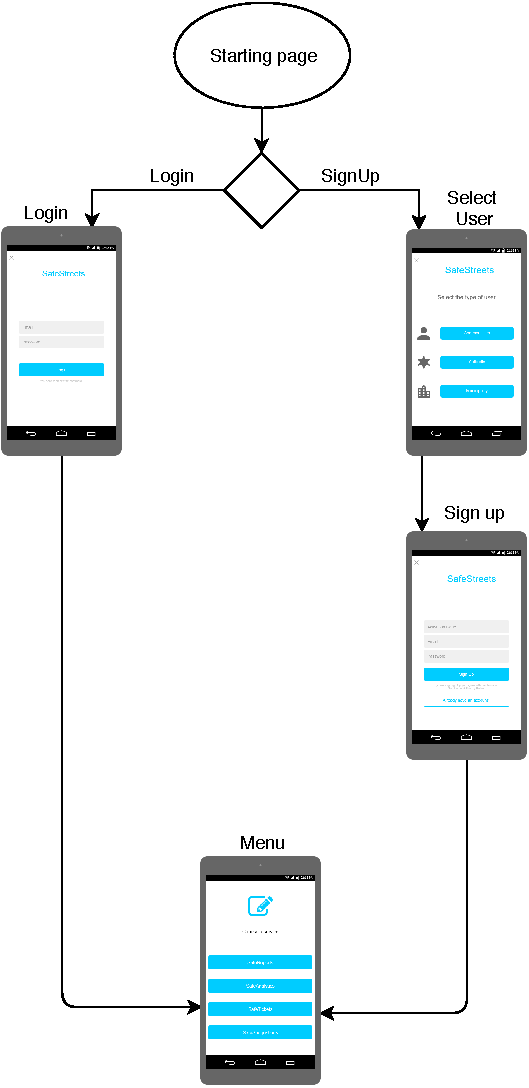
\includegraphics[]{resources/UXflow/lux}
\caption{ The user decides to login or sign-up. }
\end{figure}

\begin{figure}[H]
\centering
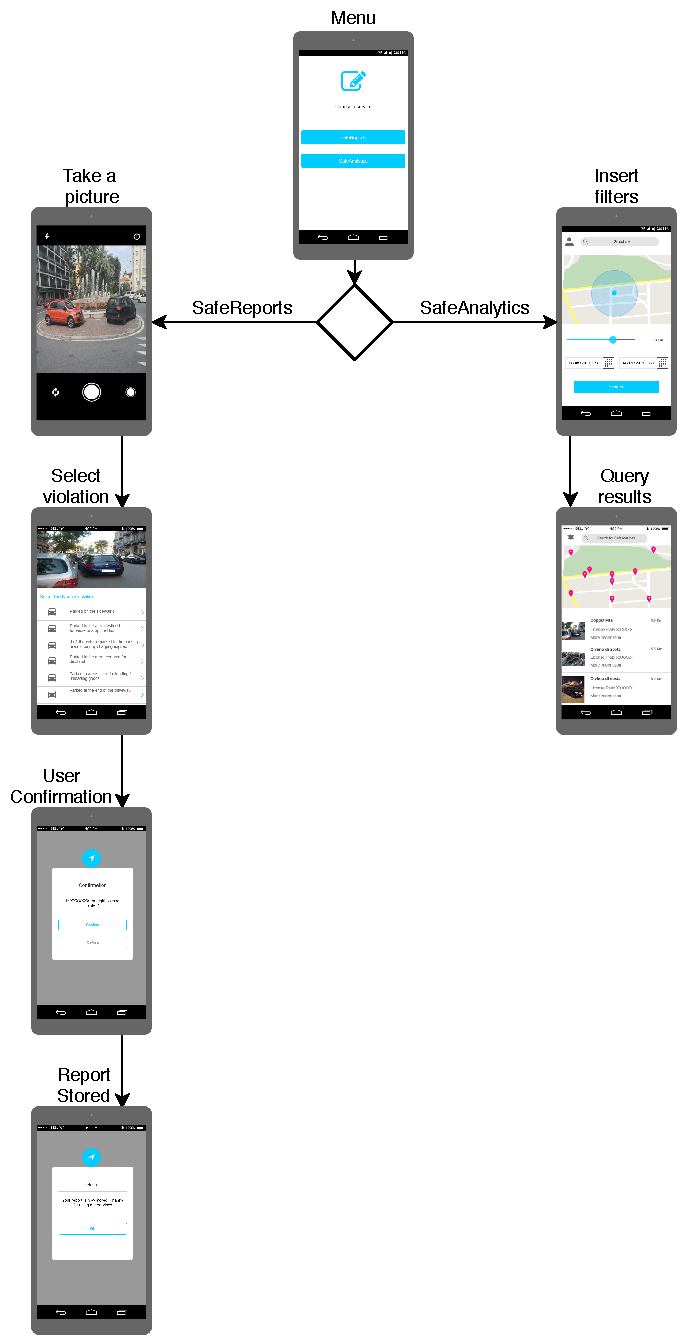
\includegraphics[width = 0.84 \textwidth]{resources/UXflow/uux}
\caption{ User choosing between SafeReports and SafeAnalytics.}
\end{figure}

\begin{figure}[H]
\centering
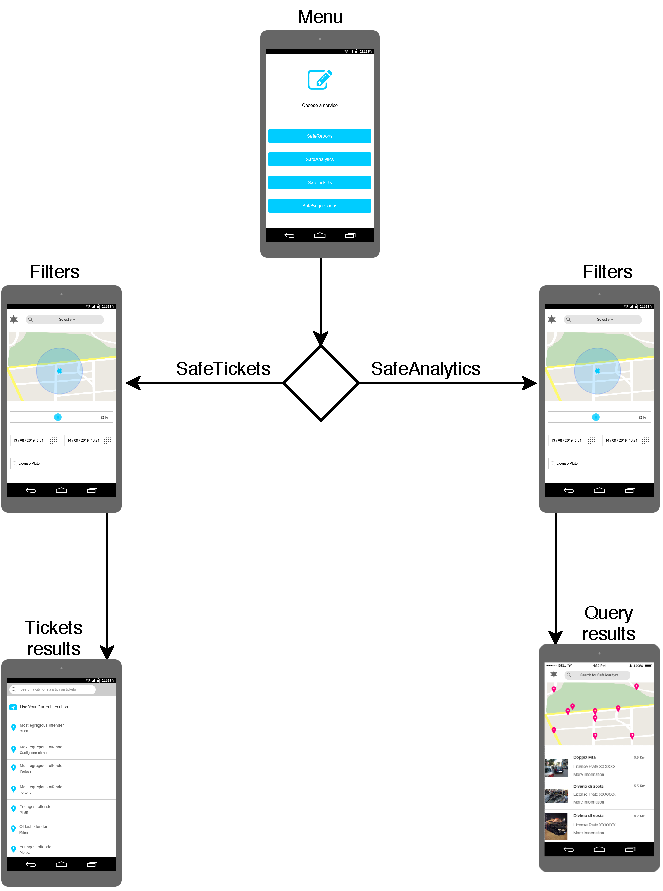
\includegraphics[]{resources/UXflow/aux}
\caption{Authorities choosing between SafeTickets and SafeAnalytics.}
\end{figure}

\begin{figure}[H]
\centering
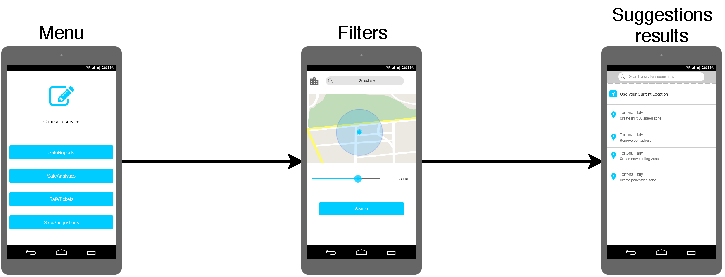
\includegraphics[]{resources/UXflow/mux}
\caption{Municipality has only SafeSuggestions as service.}
\end{figure}

The UX diagrams represent the flow of the most important user interactions with the SafeStreets app. The login sign-up diagram is unique since the distinction between the different types of users is not relevant yet. The other distinct diagrams show the different services that are available for each type of user. The UX diagrams represent the transitions between the distinct mockups. 
Other less important interactions were omitted to improve the readability of the diagrams.


\end{document}